\documentclass[11pt,aspectratio=43]{beamer}
\usepackage[utf8]{inputenc}
\usepackage{amsmath, amsfonts, amssymb, amsthm}
\usepackage[T1]{fontenc}
\usepackage{lmodern}
\usepackage{xcolor}
\usepackage{setspace}
\usepackage{booktabs}
\usepackage{multirow}
\usepackage{graphicx}
\usepackage{tikz}
% \usetikzlibrary{decorations}
\usetikzlibrary{decorations.pathreplacing, intersections, positioning}
\usepackage{ulem}
\usepackage{hyperref}
\usepackage{booktabs}
\usepackage{babel}
\usepackage{makecell}
\usepackage[para,online,flushleft]{threeparttable}
\usepackage{pdfpages}
\usepackage{tcolorbox}
\usepackage{bm}
\usepackage{appendixnumberbeamer}
\usepackage{natbib} \usepackage{caption}
\captionsetup[figure]{labelformat=empty}% redefines the caption setup of the figures environment in the beamer class.
\usetheme[compress]{Boadilla}
\usecolortheme{default}
\useoutertheme{miniframes}
\usefonttheme[onlymath]{serif}

\newcommand{\jump}[2]{\hyperlink{#1}{\beamerbutton{#2}}}
\newcommand{\orange}[1]{\textcolor{orange}{#1}}
\newcommand{\red}[1]{\textcolor{red}{#1}}

\setbeamertemplate{itemize item}{\raisebox{0.1em}{\scalebox{0.7}{$\blacksquare$}}}
\setbeamertemplate{itemize subitem}[circle]
\setbeamertemplate{itemize subsubitem}{--}
\setbeamercolor{itemize item}{fg=black}
\setbeamercolor{itemize subitem}{fg=black}
\setbeamercolor{itemize subsubitem}{fg=black}
\setbeamercolor{item projected}{bg=darkgray,fg=white}
\definecolor{blue}{rgb}{0.2, 0.2, 0.7}
\setbeamercolor{alerted text}{fg=blue}
\setbeamertemplate{enumerate items}[circle]


\setbeamertemplate{headline}{}

%==========================================
\let\olditemize=\itemize
\let\endolditemize=\enditemize
\renewenvironment{itemize}{\olditemize \itemsep1em}{\endolditemize}
\let\oldenumerate=\enumerate
\let\endoldenumerate=\endenumerate
\renewenvironment{enumerate}{\oldenumerate \itemsep1em}{ \endoldenumerate}

\DeclareMathOperator*{\argmax}{\arg\!\max}
\DeclareMathOperator*{\E}{\mathbb{E}}
\DeclareMathOperator*{\var}{\rm Var}
\DeclareMathOperator*{\cov}{\rm Cov}

\theoremstyle{definition}
\newtheorem{assume}{Assumption}
\newtheorem{lem}{Lemma}
\newtheorem{proposition}{Proposition}
\newtheorem{thm}{Theorem}
\newtheorem{corol}{Corollary}

\begin{document}
    \title[Lecture 18]{Lecture 18 \\ The Real Business Cycle Model \\ Part 5: Application and Matching Data}
    \author[Hui-Jun Chen]{Hui-Jun Chen}
    \institute[OSU]{The Ohio State University}
    % \date{\today}
    \date{\today}
    \setbeamertemplate{navigation symbols}{}
    \setstretch{1.2}

%-------------------------------------------------------
{
%	\usebackgroundtemplate{\includegraphics[width=1\paperwidth]{../EveningSky_cropped_edit43_bright.jpg}}
    \begin{frame}
% \vspace{3em}
        \centering
%		{\footnotesize 	ECON 4002 Intermediate Macroeconomic Theory}
        \maketitle
% \vspace{-1.5em}
% \centering
% \includegraphics[width=0.55\linewidth]{Pictures/houses.jpeg}


    \end{frame}
}

% -------------------------------------------
\setbeamertemplate{headline}
{
\setbeamercolor{section in head/foot}{fg=black, bg=white}
\vskip1em \tiny \insertsectionnavigationhorizontal{1\paperwidth}{\hspace{0.50\paperwidth}}{}
}
%------------------------------------------


\begin{frame}{Overview}
\label{slide:Overview}
    \begin{itemize}
        \item Recall that in Lecture 13, there is no production in dynamic model.
        \item The following $ 5 $ lectures is for \textbf{Real Business Cycle} (RBC) model:
        \begin{itemize}
            \item Lecture 14: consumer
            \item Lecture 15: firm
            \item Lecture 16: competitive equilibrium
            \item Lecture 17: formal example
            \item Lecture 18: application to bring RBC to data
        \end{itemize}
    \end{itemize}
\end{frame}

\section{z $ \uparrow  $}
\label{sec:z____uparrow___}

\begin{frame}{Analysis on $ z \uparrow  $}
\label{slide:Analysis_on___z__uparrow___}
    Suppose \alert{current TFP} increases from $ z_{1} $ to $ z_{2} $, $ z_{2} > z_{1} $
    \begin{itemize}
        \item \alert{labor demand} (firm): $ z \uparrow  $ $ \Rightarrow  $ $ MPN \uparrow  $, and thus $ N_{D, 2} > N_{D, 1}, \forall w $
        \item \alert{labor supply} (consumer): no direct effect, but $ r^{*} \downarrow  $ leads to $ N_{S}( r )  $ shifts in
        \item \alert{labor market clearing}: demand $ \uparrow  $, $ w \uparrow  $, and $ N^{*}( r ) \uparrow $, hold $ r $ fixed
        \item \alert{output supply}: shifts out $ \because $ labor market, $ Y_{S, 2} ( r ) > Y_{S, 1}( r ), \forall r$
        \item \alert{output demand}: no effect, only move along the curve, because
        \begin{itemize}
            \item firm: current TFP is not changing optimal investment schedule
            \item consumer: no direct effect
            \item government: no direct effect
        \end{itemize}
    \end{itemize}
\end{frame}

\begin{frame}{Equilibrium Effects of $ z \uparrow  $}
\label{slide:Equilibrium_Effects_of___z__uparrow___}
    \begin{columns}
        \begin{column}{0.5\textwidth}
            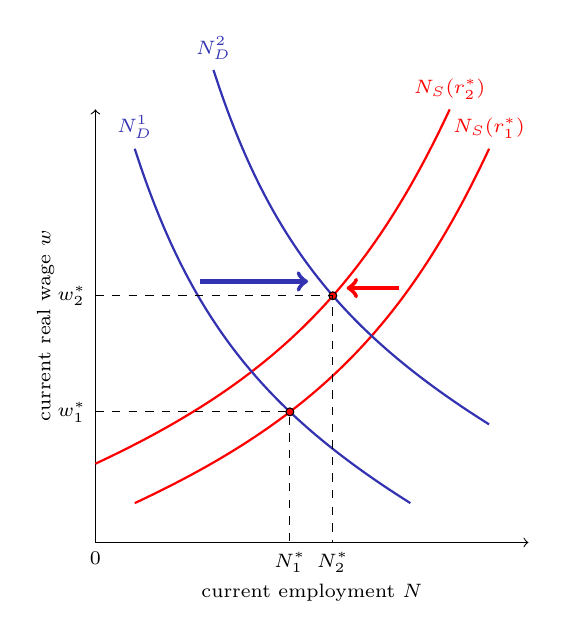
\begin{tikzpicture}[domain=0:5]
                \tikzstyle{every node}=[font=\scriptsize]
                \pgfmathsetmacro{\x}{5};
                \pgfmathsetmacro{\y}{5};
                % \draw[very thin,color=gray, step=0.1] (0,0) grid (\x, \y); % gray grid
                \draw[->] (0,0) node[below]{ $ 0 $  } -- node[below, yshift = -0.4cm]{current employment $ N $} (\x + 0.5,0) ;   % label x axis
                \draw[->] (0,0) -- node[above, rotate=90, yshift = 0.4cm]{current real wage $w$} (0,\y + 0.5) ;   % label y axis
                \draw[thick, red, name path = aa]
                    (\x, \y)
                    node[above]{$N_{S}( r_{1}^{*} )$}
                    to[bend left=20]
                    node[pos=0.3] (AA) {}
                    (0.5, 0.5);
                \draw[thick, red, xshift = -0.5cm, yshift = 0.5cm, name path = dd]
                    (\x, \y)
                    node[above]{$N_{S}( r_{2}^{*} )$}
                    to[bend left=20]
                    (0.5, 0.5);
                \draw[thick, blue, name path = bb]
                    (0.5, \y)
                    node[above]{$N_{D}^{1}$}
                    to[bend right=20]
                    node[pos=0.3] (BB) {}
                    (4, 0.5);
                \draw[thick, blue, xshift = 1cm, yshift = 1cm, name path = cc]
                    (0.5, \y)
                    node[above]{$N_{D}^{2}$}
                    to[bend right=20]
                    (4, 0.5);
                \path[name intersections={of=aa and bb, by=b}];
                \path[name intersections={of=dd and cc, by=c}];
                \node[draw,fill=red,circle,inner sep=1pt] at (b) {};
                \node[draw,fill=red,circle,inner sep=1pt] at (c) {};
                \draw[->, ultra thick, blue] (BB) -- ++(1.5, 0);
                \draw[->, ultra thick, red] (AA) -- ++(-0.8, 0);
                \path (b); \pgfgetlastxy{\xcoord}{\ycoord};
                \coordinate (b_x) at (\xcoord, 0);
                \coordinate (b_y) at (0, \ycoord);
                \path (c); \pgfgetlastxy{\xcoord}{\ycoord};
                \coordinate (c_x) at (\xcoord, 0);
                \coordinate (c_y) at (0, \ycoord);
                \draw[dashed] (b_y) node[left]{$w_{1}^{*}$}  -- (b) -- (b_x) node[below]{$N_{1}^{*}$};
                \draw[dashed] (c_y) node[left]{$w_{2}^{*}$}  -- (c) -- (c_x) node[below]{$N_{2}^{*}$};

            \end{tikzpicture}
        \end{column}
        \begin{column}{0.5\textwidth}

            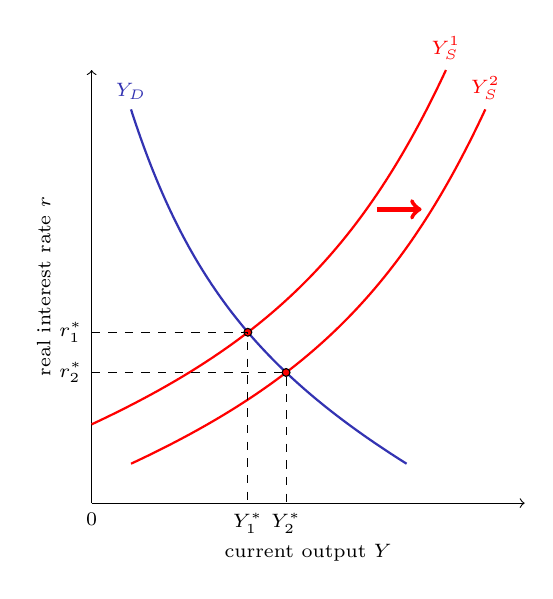
\begin{tikzpicture}[domain=0:5]
                \tikzstyle{every node}=[font=\scriptsize]
                \pgfmathsetmacro{\x}{5};
                \pgfmathsetmacro{\y}{5};
                % \draw[very thin,color=gray, step=0.1] (0,0) grid (\x, \y); % gray grid
                \draw[->] (0,0) node[below] {$ 0 $} -- node[below, yshift = -0.4cm]{current output $ Y $} (\x + 0.5,0) ;   % label x axis
                \draw[->] (0,0) -- node[above, rotate=90, yshift = 0.4cm]{real interest rate $r$} (0,\y + 0.5) ;   % label y axis
                \draw[thick, red, name path = aa]
                    (\x, \y)
                    node[above]{$Y_{S}^{2}$}
                    to[bend left=20]
                    (0.5, 0.5);
                \draw[thick, red, xshift = -0.5cm, yshift = 0.5cm, name path = cc]
                    (\x, \y)
                    node[above]{$Y_{S}^{1}$}
                    to[bend left=20]
                    node[pos=0.3] (AA) {}
                    (0.5, 0.5);
                \draw[thick, blue, name path = bb]
                    (0.5, \y)
                    node[above]{$Y_{D}$}
                    to[bend right=20]
                    (4, 0.5);
                \path[name intersections={of=aa and bb, by=a}];
                \path[name intersections={of=bb and cc, by=c}];
                \node[draw,fill=red,circle,inner sep=1pt] at (a) {};
                \node[draw,fill=red,circle,inner sep=1pt] at (c) {};
                \draw[->, ultra thick, red] (AA) -- ++(0.7, 0);
                \path (a); \pgfgetlastxy{\xcoord}{\ycoord};
                \coordinate (a_x) at (\xcoord, 0);
                \coordinate (a_y) at (0, \ycoord);
                \path (c); \pgfgetlastxy{\xcoord}{\ycoord};
                \coordinate (c_x) at (\xcoord, 0);
                \coordinate (c_y) at (0, \ycoord);
                \draw[dashed] (a_y) node[left]{$r_{2}^{*}$}  -- (a) -- (a_x) node[below]{$Y_{2}^{*}$};
                \draw[dashed] (c_y) node[left]{$r_{1}^{*}$}  -- (c) -- (c_x) node[below]{$Y_{1}^{*}$};
            \end{tikzpicture}
        \end{column}
    \end{columns}
\end{frame}

\begin{frame}{Taking Stock: $ z \uparrow  $}
\label{slide:Taking_Stock____z__uparrow___}
    Output supply curve shifts out, while output demand remain the same
    \begin{itemize}
        \item output $ \uparrow  $, $ Y_{2} > Y_{1} $
        \item real interest rate $ \downarrow  $, $ r_{2} < r_{1} $
        \item decreases in $ r $ make labor supply shifts in
        \begin{itemize}
            \item saving $ S $ become less desirable, so no need to work that much
        \end{itemize}
        \item wage increase because of the shifts in demand and supply
        \item effect on $ N^{*} $ is theoretically ambiguous, yet data shows that the effect of intertemporal substitution of leisure ($N_{S} \downarrow $) is small
    \end{itemize}
    Recall \textbf{business cycle facts}: procyclical labor, real wage, and average labor productivity.

    All consistent with model prediction!

\end{frame}

\section{$z' \uparrow $}
\label{sec:_z___uparrow__}

\begin{frame}{Analysis on $ z' \uparrow  $}
\label{slide:Analysis_on___z___uparrow___}
    \begin{itemize}
        \item \alert{labor demand}: no direct effect
        \item \alert{labor supply}: no direct effect, yet $ r \uparrow  $ cause supply to shift to the right
        \item \alert{output supply}: no direct effect
        \item \alert{output demand}: higher $ z' $ $ \Rightarrow  $ higher $ MPK' $ $ \Rightarrow  $ firm's investment demand is higher $ \Rightarrow  $ demand shifts to the right
        \begin{itemize}
            \item no direct effect from consumer and government
        \end{itemize}
    \end{itemize}
\end{frame}

\begin{frame}{Equilibrium Effect of $ z' \uparrow  $}
\label{slide:Equilibrium_Effect_of___z___uparrow___}
    \begin{columns}
        \begin{column}{0.5\textwidth}
            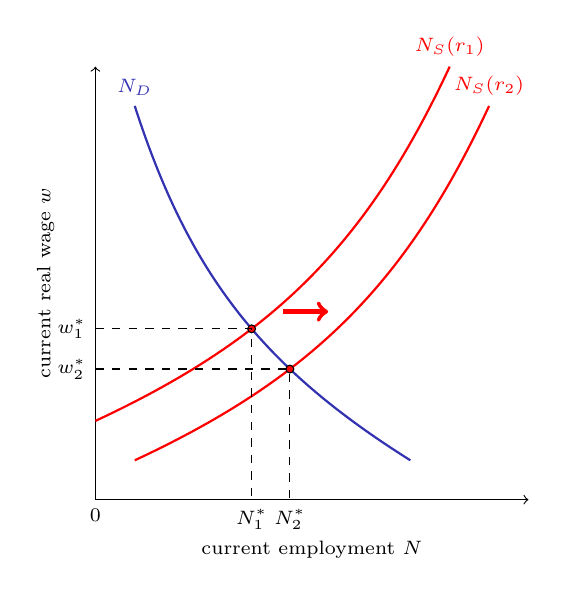
\begin{tikzpicture}[domain=0:5]
                \tikzstyle{every node}=[font=\scriptsize]
                \pgfmathsetmacro{\x}{5};
                \pgfmathsetmacro{\y}{5};
                % \draw[very thin,color=gray, step=0.1] (0,0) grid (\x, \y); % gray grid
                \draw[->] (0,0) node[below]{ $ 0 $  } -- node[below, yshift = -0.4cm]{current employment $ N $} (\x + 0.5,0) ;   % label x axis
                \draw[->] (0,0) -- node[above, rotate=90, yshift = 0.4cm]{current real wage $w$} (0,\y + 0.5) ;   % label y axis
                \draw[thick, red, xshift = -0.5cm, yshift = 0.5cm, name path = aaa]
                    (\x, \y)
                    node[above]{$N_{S}( r_{1} )$}
                    to[bend left=20]
                    node[pos=0.6] (AA) {}
                    (0.5, 0.5);
                \draw[thick, red, name path = aa]
                    (\x, \y)
                    node[above]{$N_{S}( r_{2} )$}
                    to[bend left=20]
                    (0.5, 0.5);
                \draw[thick, blue, name path = bb]
                    (0.5, \y)
                    node[above]{$N_{D}$}
                    to[bend right=20]
                    (4, 0.5);
                \path[name intersections={of=aa and bb, by=b}];
                \path[name intersections={of=aaa and bb, by=bb}];
                \node[draw,fill=red,circle,inner sep=1pt] at (b) {};
                \node[draw,fill=red,circle,inner sep=1pt] at (bb) {};
                \draw[->, ultra thick, red] (AA) -- ++(0.7, 0);
                \path (bb); \pgfgetlastxy{\xcoord}{\ycoord};
                \coordinate (bb_x) at (\xcoord, 0);
                \coordinate (bb_y) at (0, \ycoord);
                \draw[dashed] (bb_y) node[left]{$w_{1}^{*}$}  -- (bb) -- (bb_x) node[below]{$N_{1}^{*}$};
                \path (b); \pgfgetlastxy{\xcoord}{\ycoord};
                \coordinate (b_x) at (\xcoord, 0);
                \coordinate (b_y) at (0, \ycoord);
                \draw[dashed] (b_y) node[left]{$w_{2}^{*}$}  -- (b) -- (b_x) node[below]{$N_{2}^{*}$};

            \end{tikzpicture}
        \end{column}
        \begin{column}{0.5\textwidth}

            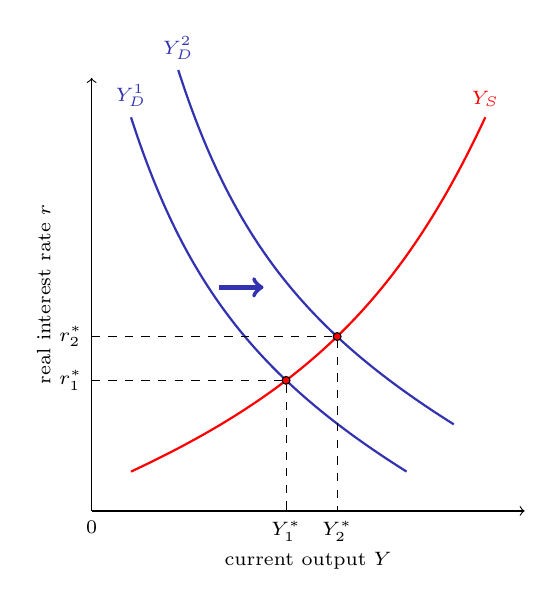
\begin{tikzpicture}[domain=0:5]
                \tikzstyle{every node}=[font=\scriptsize]
                \pgfmathsetmacro{\x}{5};
                \pgfmathsetmacro{\y}{5};
                % \draw[very thin,color=gray, step=0.1] (0,0) grid (\x, \y); % gray grid
                \draw[->] (0,0) node[below]{ $ 0 $  } -- node[below, yshift = -0.4cm]{current output $ Y $} (\x + 0.5,0) ;   % label x axis
                \draw[->] (0,0) -- node[above, rotate=90, yshift = 0.4cm]{real interest rate $r$} (0,\y + 0.5) ;   % label y axis
                \draw[thick, red, name path = aa]
                    (\x, \y)
                    node[above]{$Y_{S}$}
                    to[bend left=20]
                    (0.5, 0.5);
                \draw[thick, blue, name path = bb]
                    (0.5, \y)
                    node[above]{$Y_{D}^{1}$}
                    to[bend right=20]
                    node[pos = 0.4] (BB) {}
                    (4, 0.5);
                \draw[thick, blue, xshift = 0.6cm, yshift = 0.6cm, name path = bbb]
                    (0.5, \y)
                    node[above]{$Y_{D}^{2}$}
                    to[bend right=20]
                    (4, 0.5);
                \path[name intersections={of=aa and bb, by=a}];
                \path[name intersections={of=aa and bbb, by=bbb}];
                \node[draw,fill=red,circle,inner sep=1pt] at (a) {};
                \node[draw,fill=red,circle,inner sep=1pt] at (bbb) {};
                \draw[->, ultra thick, blue] (BB) -- ++(0.7, 0);
                \path (a); \pgfgetlastxy{\xcoord}{\ycoord};
                \coordinate (a_x) at (\xcoord, 0);
                \coordinate (a_y) at (0, \ycoord);
                \draw[dashed] (a_y) node[left]{$r_{1}^{*}$}  -- (a) -- (a_x) node[below]{$Y_{1}^{*}$};
                \path (bbb); \pgfgetlastxy{\xcoord}{\ycoord};
                \coordinate (bbb_x) at (\xcoord, 0);
                \coordinate (bbb_y) at (0, \ycoord);
                \draw[dashed] (bbb_y) node[left]{$r_{2}^{*}$}  -- (bbb) -- (bbb_x) node[below]{$Y_{2}^{*}$};

            \end{tikzpicture}
        \end{column}
    \end{columns}
\end{frame}

\section{$K \downarrow  $}
\label{sec:K____downarrow___}

\begin{frame}{Analysis on Destruction of Initial Capital $ K \downarrow  $}
\label{slide:Analysis_on_Destruction_of_Initial_Capital___K__downarrow___}
Suppose a natural disaster destroys some initial capital: $ K_{1} \rightarrow K_{2} $, where $ K_{2} < K_{1} $.
\begin{itemize}
    \item \alert{labor demand}: $ K \downarrow  $ $ \Rightarrow  $ $ MPN \downarrow  $ $ \Rightarrow  $ $ N_{D}^{2}( w ) < N_{D}^{1} ( w ), \forall w $
    \item \alert{labor supply}: no direct effect, but $ r^{*} \uparrow  $ $ \Rightarrow  $ $ N_{S} ( r ) \downarrow  $
    \item \alert{labor market clearing}: lower wage and quantity of labor, hold $ r $ fixed
    \item \alert{output supply}: shifts in, $ \because $ labor market effects, $ Y_{S}^{2}( r ) < Y_{S}^{1}( r ), \forall r $
    \item \alert{output demand}: shifts out, because
    \begin{itemize}
        \item firm: $ K \downarrow $, so must $ I_{D} \uparrow  $ to meet same amount of $ K' $
        \begin{itemize}
            \item remember capital accumulation process $K' = I_{D} + ( 1-\delta ) K$
        \end{itemize}
        \item consumer and government have no direct effects
    \end{itemize}
\end{itemize}
\end{frame}

\begin{frame}{Equilibrium Effect of $ K \downarrow  $}
\label{slide:Equilibrium_Effect_of___K__downarrow___}
    \begin{columns}
        \begin{column}{0.5\textwidth}
            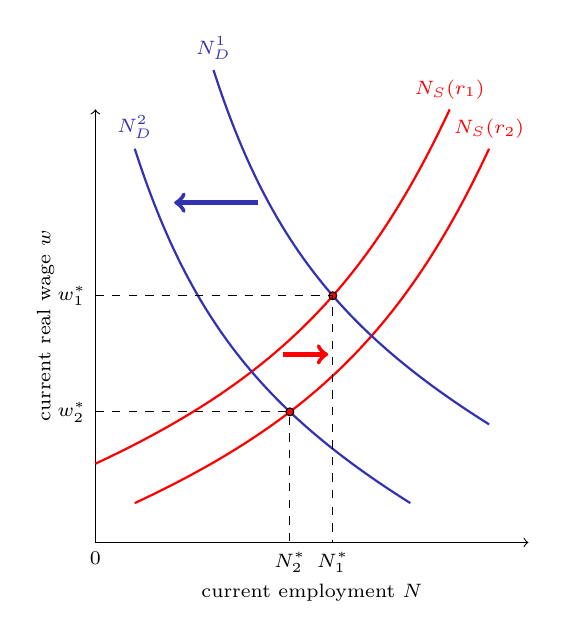
\begin{tikzpicture}[domain=0:5]
                \tikzstyle{every node}=[font=\scriptsize]
                \pgfmathsetmacro{\x}{5};
                \pgfmathsetmacro{\y}{5};
                % \draw[very thin,color=gray, step=0.1] (0,0) grid (\x, \y); % gray grid
                \draw[->] (0,0) node[below]{ $ 0 $  } -- node[below, yshift = -0.4cm]{current employment $ N $} (\x + 0.5,0) ;   % label x axis
                \draw[->] (0,0) -- node[above, rotate=90, yshift = 0.4cm]{current real wage $w$} (0,\y + 0.5) ;   % label y axis
                \draw[thick, red, xshift = -0.5cm, yshift = 0.5cm, name path = aaa]
                    (\x, \y)
                    node[above]{$N_{S}( r_{1} )$}
                    to[bend left=20]
                    node[pos=0.6] (AA) {}
                    (0.5, 0.5);
                \draw[thick, red, name path = aa]
                    (\x, \y)
                    node[above]{$N_{S}( r_{2} )$}
                    to[bend left=20]
                    (0.5, 0.5);
                \draw[thick, blue, xshift = 1cm, yshift = 1cm, name path = bbb]
                    (0.5, \y)
                    node[above]{$N_{D}^{1}$}
                    to[bend right=20]
                    node[pos = 0.3] (BB) {}
                    (4, 0.5);
                \draw[thick, blue, name path = bb]
                    (0.5, \y)
                    node[above]{$N_{D}^{2}$}
                    to[bend right=20]
                    (4, 0.5);
                \path[name intersections={of=aa and bb, by=b}];
                \path[name intersections={of=aaa and bbb, by=bb}];
                \node[draw,fill=red,circle,inner sep=1pt] at (b) {};
                \node[draw,fill=red,circle,inner sep=1pt] at (bb) {};
                \draw[->, ultra thick, red] (AA) -- ++(0.7, 0);
                \draw[->, ultra thick, blue] (BB) -- ++(-1.2, 0);
                \path (bb); \pgfgetlastxy{\xcoord}{\ycoord};
                \coordinate (bb_x) at (\xcoord, 0);
                \coordinate (bb_y) at (0, \ycoord);
                \draw[dashed] (bb_y) node[left]{$w_{1}^{*}$}  -- (bb) -- (bb_x) node[below]{$N_{1}^{*}$};
                \path (b); \pgfgetlastxy{\xcoord}{\ycoord};
                \coordinate (b_x) at (\xcoord, 0);
                \coordinate (b_y) at (0, \ycoord);
                \draw[dashed] (b_y) node[left]{$w_{2}^{*}$}  -- (b) -- (b_x) node[below]{$N_{2}^{*}$};

            \end{tikzpicture}
        \end{column}
        \begin{column}{0.5\textwidth}

            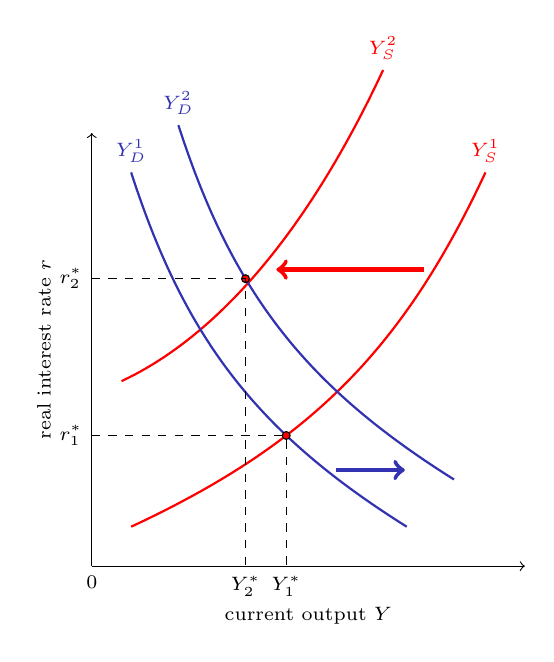
\begin{tikzpicture}[domain=0:5]
                \tikzstyle{every node}=[font=\scriptsize]
                \pgfmathsetmacro{\x}{5};
                \pgfmathsetmacro{\y}{5};
                % \draw[very thin,color=gray, step=0.1] (0,0) grid (\x, \y); % gray grid
                \draw[->] (0,0) node[below]{ $ 0 $  } -- node[below, yshift = -0.4cm]{current output $ Y $} (\x + 0.5,0) ;   % label x axis
                \draw[->] (0,0) -- node[above, rotate=90, yshift = 0.4cm]{real interest rate $r$} (0,\y + 0.5) ;   % label y axis
                \draw[thick, red, name path = aa]
                    (\x, \y)
                    node[above]{$Y_{S}^{1}$}
                    to[bend left=20]
                    node[pos = 0.2] (AA) {}
                    (0.5, 0.5);
                \draw[thick, red, xshift = -1.3cm, yshift = 1.3cm, name path = aaa, shorten >= 1.3cm]
                    (\x, \y)
                    node[above]{$Y_{S}^{2}$}
                    to[bend left=20]
                    (0.5, 0.5);
                \draw[thick, blue, name path = bb]
                    (0.5, \y)
                    node[above]{$Y_{D}^{1}$}
                    to[bend right=20]
                    node[pos = 0.8] (BB) {}
                    (4, 0.5);
                \draw[thick, blue, xshift = 0.6cm, yshift = 0.6cm, name path = bbb]
                    (0.5, \y)
                    node[above]{$Y_{D}^{2}$}
                    to[bend right=20]
                    (4, 0.5);
                \path[name intersections={of=aa and bb, by=a}];
                \path[name intersections={of=aaa and bbb, by=bbb}];
                \node[draw,fill=red,circle,inner sep=1pt] at (a) {};
                \node[draw,fill=red,circle,inner sep=1pt] at (bbb) {};
                \draw[->, ultra thick, blue] (BB) -- ++(1, 0);
                \draw[->, ultra thick, red] (AA) -- ++(-2, 0);
                \path (a); \pgfgetlastxy{\xcoord}{\ycoord};
                \coordinate (a_x) at (\xcoord, 0);
                \coordinate (a_y) at (0, \ycoord);
                \draw[dashed] (a_y) node[left]{$r_{1}^{*}$}  -- (a) -- (a_x) node[below]{$Y_{1}^{*}$};
                \path (bbb); \pgfgetlastxy{\xcoord}{\ycoord};
                \coordinate (bbb_x) at (\xcoord, 0);
                \coordinate (bbb_y) at (0, \ycoord);
                \draw[dashed] (bbb_y) node[left]{$r_{2}^{*}$}  -- (bbb) -- (bbb_x) node[below]{$Y_{2}^{*}$};

            \end{tikzpicture}
        \end{column}
    \end{columns}
\end{frame}

\section{$G \uparrow $}
\label{sec:_G__uparrow__}

\begin{frame}{Analysis on Government Spending Increase $ G \uparrow  $}
\label{slide:Analysis_on_Government_Spending_Increase___G__uparrow___}
    Suppose $ G \uparrow  $, holding $ G' $ fixed. This is more complicated...
    \begin{itemize}
        \item \alert{example}: wartime spending (WWII), Stimulus in recession (COVID check)
    \end{itemize}
    Need to trace individual decisions and market clearing conditions to find \textbf{overall equilibrium effect}.
    \begin{itemize}
        \item \alert{simplification}: assume $ MPC $ is constant
        \item \alert{interpretation}: slope $ <1 $ in output demand curve
        \item \alert{example}: $ U( C, C' ) = \ln C + \beta \ln C' $ $ \Rightarrow  $ $ C' = \beta ( 1+r ) C $, which implies
        %
        \begin{equation*}
            C = \frac{1}{1+\beta} \left(
                Y - T + \frac{Y' - T'}{1+r}
            \right)
            \Rightarrow  \frac{dC}{dY} = \frac{1}{1+\beta}
        \end{equation*}
        %
    \end{itemize}
\end{frame}

\begin{frame}{Impact on Output Demand}
\label{slide:Impact_on_Output_Demand}
    $ G \uparrow  $ causes \alert{a $ \Delta $ amount of shift in the output demand curve}. How big is $ \Delta $, and where do the change comes from?
    \begin{enumerate}
        \item direct effect: $ G_{2} - G_{1} > 0 $
        \item indirect effect: increase in taxes decreases the consumption
        \begin{itemize}
            \item $ \because G_{2} > G_{1} $, $ T_{2} + \frac{T'_{2}}{1+r} > T_{1} + \frac{T'_{1}}{1+r} $, and thus consumer's income $ \downarrow  $ by the amount of $ G_{2} - G_{1} $.
            \item effect on consumption: $ MPC \times ( G_{2} - G_{1} ) $
        \end{itemize}
        \item indirect effect: consumer perceives as $ Y_{D} $ changes $ \Delta $ amount, and thus consumption changes.
        \begin{itemize}
            \item translate to consumption: $ MPC \times \Delta $
        \end{itemize}
    \end{enumerate}
    \begin{center}
        $ \displaystyle \Delta = G_{2} - G_{1} + MPC \times ( G_{2} - G_{1} ) + MPC \times \Delta \Rightarrow \alert{\Delta = G_{2} - G_{1}}$
    \end{center}
    note: more complicated if MPC is not constant, or varies across people!
\end{frame}

\begin{frame}{Impact on Output Demand (Cont.)}
\label{slide:Impact_on_Output_Demand__Cont__}
The \alert{elasticity} of output demand with respect to government spending is defined as the \textbf{demand multiplier}:
\begin{center}
    $ \displaystyle m_{D} = \frac{\Delta}{G_{2} - G_{1}} = 1 $
\end{center}
\begin{itemize}
    \item implication: rightward shift of the demand curve is exactly 1-1
    \item because of 1-1 relationship, we know \alert{$ Y_{D}^{2}( r ) = Y_{D}^{2}( r ) + \Delta $}
\end{itemize}

\end{frame}

\begin{frame}{Impact on Output Supply}
\label{slide:Impact_on_Output_Supply}
    \begin{itemize}
        \item \alert{labor demand}: no effect
        \item \alert{labor supply}: outward shift, $ \because $ wealth effect of $ T, T' \uparrow  $
        \begin{itemize}
            \item holding $ r $ fixed, $ N_{S}^{2}( r_{1} ) > N_{S}^{1} ( r_{1} ) $
            \item in equilibrium of next slide, $ r^{*} \uparrow  $, and thus saving become desirable, $ N_{S}^{2}( r_{2} ) > N_{S}^{2} ( r_{1} ) $
        \end{itemize}
        \item \alert{output supply}: shifts out, given labor supply shifts
    \end{itemize}
    Combine effects: $ Y^{*} \uparrow  $, $ N^{*} \uparrow  $, $ w^{*} \downarrow  $, yet $ r^{*} $ depends on the amount of movement for both demand and supply.

\end{frame}


\begin{frame}{Equilibrium Effect of $ G \uparrow  $}
\label{slide:Equilibrium_Effect_of___G__uparrow___}
    \begin{columns}
        \begin{column}{0.5\textwidth}
            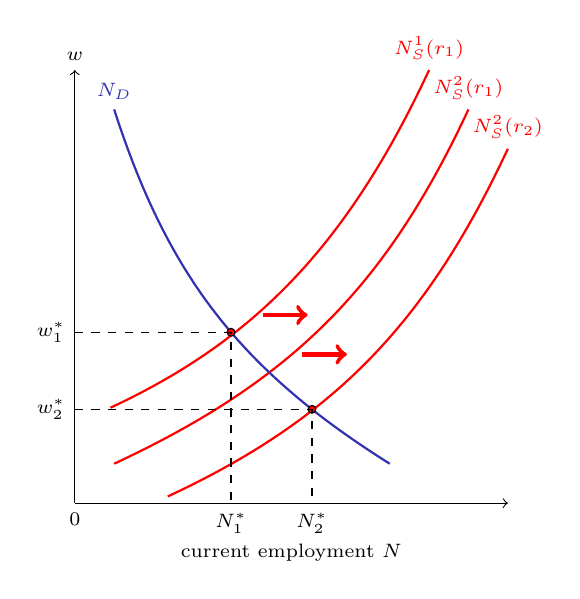
\begin{tikzpicture}[domain=0:5]
                \tikzstyle{every node}=[font=\scriptsize]
                \pgfmathsetmacro{\x}{5};
                \pgfmathsetmacro{\y}{5};
                % \draw[very thin,color=gray, step=0.1] (0,0) grid (\x, \y); % gray grid
                \draw[->] (0,0) node[below]{ $ 0 $  } -- node[below, yshift = -0.4cm]{current employment $ N $} (\x + 0.5,0) ;   % label x axis
                \draw[->] (0,0) -- (0,\y + 0.5) node[above]{$w$} ;   % label y axis
                \draw[thick, red, xshift = -0.5cm, yshift = 0.5cm, name path = aaa, shorten >= 0.5cm]
                    (\x, \y)
                    node[above]{$N_{S}^{1}( r_{1} )$}
                    to[bend left=20]
                    node[pos=0.6] (AA) {}
                    (0.5, 0.5);
                \draw[thick, red, name path = aa]
                    (\x, \y)
                    node[above]{$N_{S}^{2}( r_{1} )$}
                    to[bend left=20]
                    node[pos=0.6] (AAA) {}
                    (0.5, 0.5);
                \draw[thick, red, xshift = 0.5cm, yshift = -0.5cm, name path = aaaa, shorten >= 0.2cm]
                    (\x, \y)
                    node[above]{$N_{S}^{2}( r_{2} )$}
                    to[bend left=20]
                    (0.5, 0.5);
                \draw[thick, blue, name path = bb]
                    (0.5, \y)
                    node[above]{$N_{D}$}
                    to[bend right=20]
                    (4, 0.5);
                \path[name intersections={of=aaaa and bb, by=b}];
                \path[name intersections={of=aaa and bb, by=bb}];
                \node[draw,fill=red,circle,inner sep=1pt] at (b) {};
                \node[draw,fill=red,circle,inner sep=1pt] at (bb) {};
                \draw[->, ultra thick, red] (AA) -- ++(0.7, 0);
                \draw[->, ultra thick, red] (AAA) -- ++(0.7, 0);
                \path (bb); \pgfgetlastxy{\xcoord}{\ycoord};
                \coordinate (bb_x) at (\xcoord, 0);
                \coordinate (bb_y) at (0, \ycoord);
                \draw[dashed] (bb_y) node[left]{$w_{1}^{*}$}  -- (bb) -- (bb_x) node[below]{$N_{1}^{*}$};
                \path (b); \pgfgetlastxy{\xcoord}{\ycoord};
                \coordinate (b_x) at (\xcoord, 0);
                \coordinate (b_y) at (0, \ycoord);
                \draw[dashed] (b_y) node[left]{$w_{2}^{*}$}  -- (b) -- (b_x) node[below]{$N_{2}^{*}$};

            \end{tikzpicture}
        \end{column}
        \begin{column}{0.5\textwidth}

            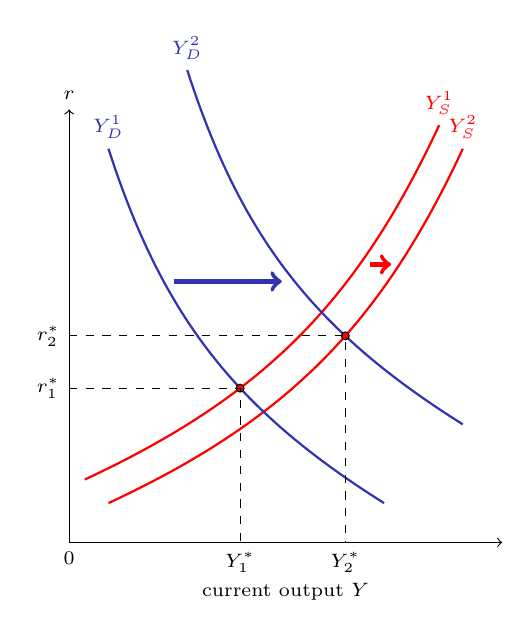
\begin{tikzpicture}[domain=0:5]
                \tikzstyle{every node}=[font=\scriptsize]
                \pgfmathsetmacro{\x}{5};
                \pgfmathsetmacro{\y}{5};
                % \draw[very thin,color=gray, step=0.1] (0,0) grid (\x, \y); % gray grid
                \draw[->] (0,0) node[below]{ $ 0 $  } -- node[below, yshift = -0.4cm]{current output $ Y $} (\x + 0.5,0) ;   % label x axis
                \draw[->] (0,0) -- (0,\y + 0.5) node[above]{$r$} ;   % label y axis
                \draw[thick, red, xshift = -0.3cm, yshift = 0.3cm, name path = aaa]
                    (\x, \y)
                    node[above]{$Y_{S}^{1}$}
                    to[bend left=20]
                    node[pos = 0.3] (AA) {}
                    (0.5, 0.5);
                \draw[thick, red, name path = aa]
                    (\x, \y)
                    node[above]{$Y_{S}^{2}$}
                    to[bend left=20]
                    (0.5, 0.5);
                \draw[thick, blue, name path = bb]
                    (0.5, \y)
                    node[above]{$Y_{D}^{1}$}
                    to[bend right=20]
                    node[pos = 0.3] (BB) {}
                    (4, 0.5);
                \draw[thick, blue, xshift = 1cm, yshift = 1cm, name path = bbb]
                    (0.5, \y)
                    node[above]{$Y_{D}^{2}$}
                    to[bend right=20]
                    (4, 0.5);
                \path[name intersections={of=aaa and bb, by=a}];
                \path[name intersections={of=aa and bbb, by=bbb}];
                \node[draw,fill=red,circle,inner sep=1pt] at (a) {};
                \node[draw,fill=red,circle,inner sep=1pt] at (bbb) {};
                \draw[->, ultra thick, blue] (BB) -- ++(1.5, 0);
                \draw[->, ultra thick, red] (AA) -- ++(0.4, 0);
                \path (a); \pgfgetlastxy{\xcoord}{\ycoord};
                \coordinate (a_x) at (\xcoord, 0);
                \coordinate (a_y) at (0, \ycoord);
                \draw[dashed] (a_y) node[left]{$r_{1}^{*}$}  -- (a) -- (a_x) node[below]{$Y_{1}^{*}$};
                \path (bbb); \pgfgetlastxy{\xcoord}{\ycoord};
                \coordinate (bbb_x) at (\xcoord, 0);
                \coordinate (bbb_y) at (0, \ycoord);
                \draw[dashed] (bbb_y) node[left]{$r_{2}^{*}$}  -- (bbb) -- (bbb_x) node[below]{$Y_{2}^{*}$};

            \end{tikzpicture}
        \end{column}
    \end{columns}
\end{frame}

\begin{frame}{Taking Stock: Output}
\label{slide:Taking_Stock__Output}
    What is the \alert{total government expenditure multiplier}?
    \begin{itemize}
        \item \alert{definition}: the \textbf{equilibrium} (as opposed to demand or supply only) ratio of increase in output to the increase in government spending.
        \item \alert{result:} must is less than 1 without ``large'' shifts in supply curve
        \begin{itemize}
            \item  shift in output demand curve is $ G_{2} - G_{1} $ for each $ r $
            \item supply curve slopes up: equilibrium effect $ < G_{2} - G_{1} $ (before shift)
            \item what determines size of supply curve shift?
            \begin{itemize}
                \item size of wealth effect on labor supply (small)
                \item size of intertemporal substitution effect on labor supply (small)
            \end{itemize}
            \item ``Keynesian'' stimulus: multiplier may be positive in recessions, but need some sort of economic inefficiency for this result.
        \end{itemize}
    \end{itemize}
\end{frame}

\begin{frame}{Taking Stock: Everything Else}
\label{slide:Taking_Stock__Everything_Else}
    Imagine supply curve is horizontal:
    \begin{itemize}
        \item equilibrium effect: $ Y_{2} - Y_{1} = G_{2} - G_{1} $, no change in $ r $
        \item would have to come from no change in consumer’s lifetime wealth, and so would induce no change in current consumption.
    \end{itemize}
    With upward slope sufficient to make $ r_{2} > r_{1} $ (empirically plausible case):
    \begin{itemize}
        \item consumption falls due to intertemporal substitution effect
        \item investment falls due to higher opportunity cost of investing in capital
        \item ``crowding out:'' government expenditures here also limit future production
        \item total: higher output, but at what cost?
    \end{itemize}
\end{frame}
\end{document}
